\documentclass{article}

\usepackage[british,UKenglish,USenglish,english,american]{babel}
\usepackage[utf8]{inputenc}
\usepackage{amsmath}
\usepackage{amssymb}
\usepackage{anysize}
\usepackage{color}
\usepackage{xcolor}
\usepackage{graphicx}
\graphicspath{ {./images/} }
\usepackage{babel,blindtext}
\usepackage{hyperref} % % package for inserting Hyperlinks
\usepackage{tikz}
\usetikzlibrary{shapes,snakes}
\usetikzlibrary{shapes.misc, shapes.arrows}
\usetikzlibrary{calc, matrix,chains,scopes,positioning,arrows,fit}


\usepackage{listings}
\lstset{
	language=C++,                	% choose the language of the code
	basicstyle=\footnotesize,       % the size of the fonts that are used for the code
	numbers= left,                 	% where to put the line-numbers
	numberstyle=\footnotesize,      % the size of the fonts that are used for the line-numbers
	stepnumber=2,                   % the step between two line-numbers. If it is 1 each line will be numbered
	numbersep=5pt,                  % how far the line-numbers are from the code
	backgroundcolor=\color{white},  % choose the background color. You must add \usepackage{color}
	showspaces=false,               % show spaces adding particular underscores
	showstringspaces=false,         % underline spaces within strings
	showtabs=false,                 % show tabs within strings adding particular underscores
	frame=single,           		% adds a frame around the code
	tabsize=2,          			% sets default tabsize to 2 spaces
	captionpos=t,          			% sets the caption-position to bottom (t=top, b=bottom)
	breaklines=true,        		% sets automatic line breaking
	breakatwhitespace=false,    	% sets if automatic breaks should only happen at whitespace
	escapeinside={\%*}{*)}          % if you want to add a comment within your code
}

\usepackage{caption}
\DeclareCaptionFont{white}{\color{white}}
\DeclareCaptionFormat{listing}{\colorbox{gray}{\parbox[c]{\textwidth}{#1#2#3}}}
\captionsetup[lstlisting]{format=listing,labelfont=white,textfont=white}

\setlength\parindent{0pt}
\setlength{\parskip}{10pt}

\marginsize{3cm}{2cm}{2cm}{2cm}

\title{Software Engineering Project}
\author{Donatas Kozlovskis, Enric Cornellà\\
		Andrey Pak,  Fernando Garcia\\
		VIBOT-8}
\date{11/12/13}

\begin{document}
\maketitle

\section{Introduction}

The present document illustrates all decisions, procedures and methodology followed during the development of the application map. But also specific documentation regarding the implementation such as diagrams or remarkable algorithms specifically designed to solve the problems from the implementation.

This document has been divided in three different main sections; the first one shows the time line followed for carrying out the project and the common decision taken regarding the two other following sections, the second section focusses on the C++ implementation and finally, the last one, focusses on the Matlab part. 

\subsection{Tools and resources}
This section shows which software has been used directly or indirectly during the whole phase of design as well as the phase of development.
In order to manage the whole our project and its tasks, we have chosen the web-based project management application \textit{Trello}.It allows to keep track of everything, from the big picture to the minute details. In this way, all kind of tasks can be divided and assigned to the people involved in the project and also can be located in different boards according to the state of development of the task as in the following image:

\begin{figure}[!h]
\centering
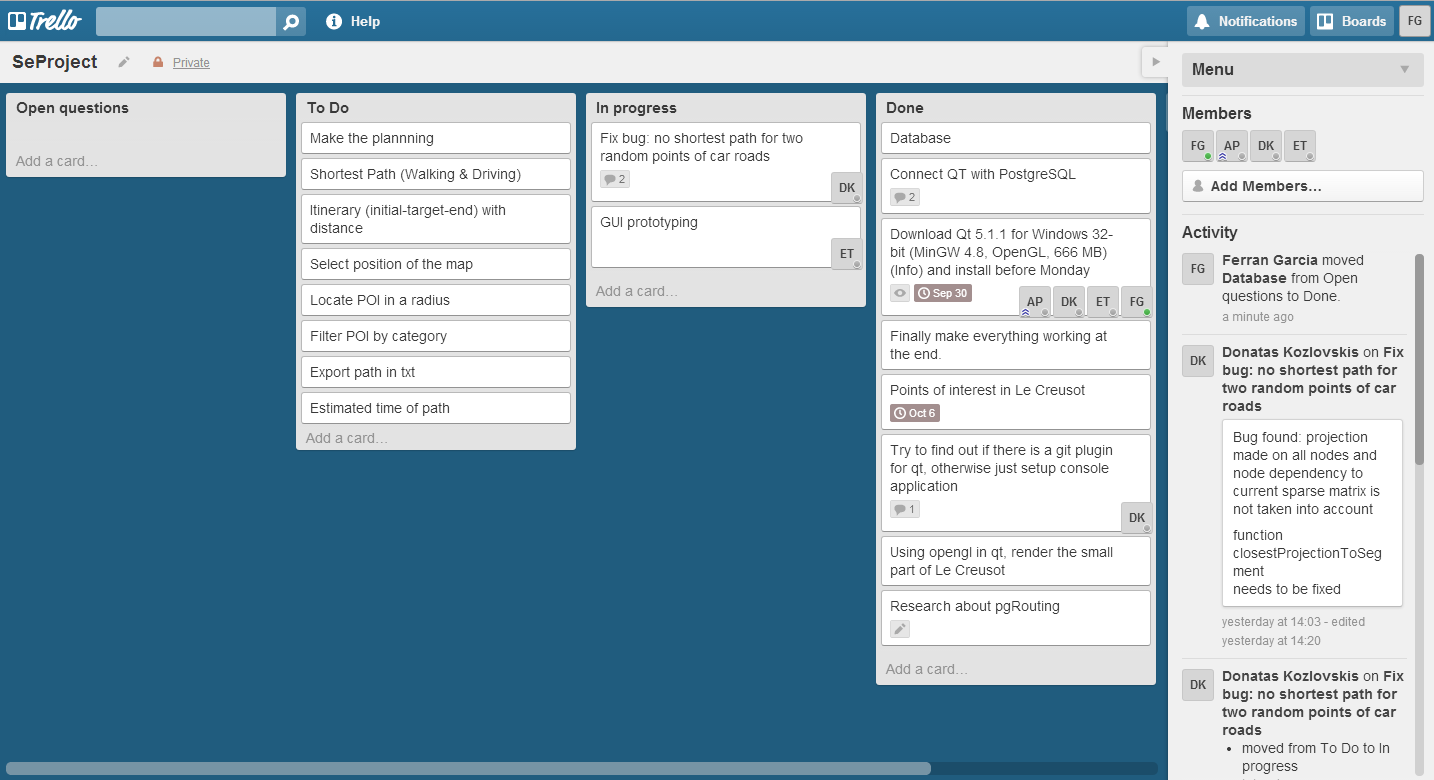
\includegraphics[width=0.68\textwidth]{trello.png}
\caption{Image of the task manager during the development process at early stages. The work is divided in four different boards with multiple drag and drop tasks and is assigned to one person}
\end{figure}

At the same time, real world meetings were not avoided. Normally we tried to establish team meeting at least once in a week. In such meetings we have discussed common problems, created good ideas or simply tried to brainstorm as many ideas as possible.Afterwards, the results of such meetings were definitely moved to the interactive board in \textit{Trello}.

\begin{figure}[!h]
\centering
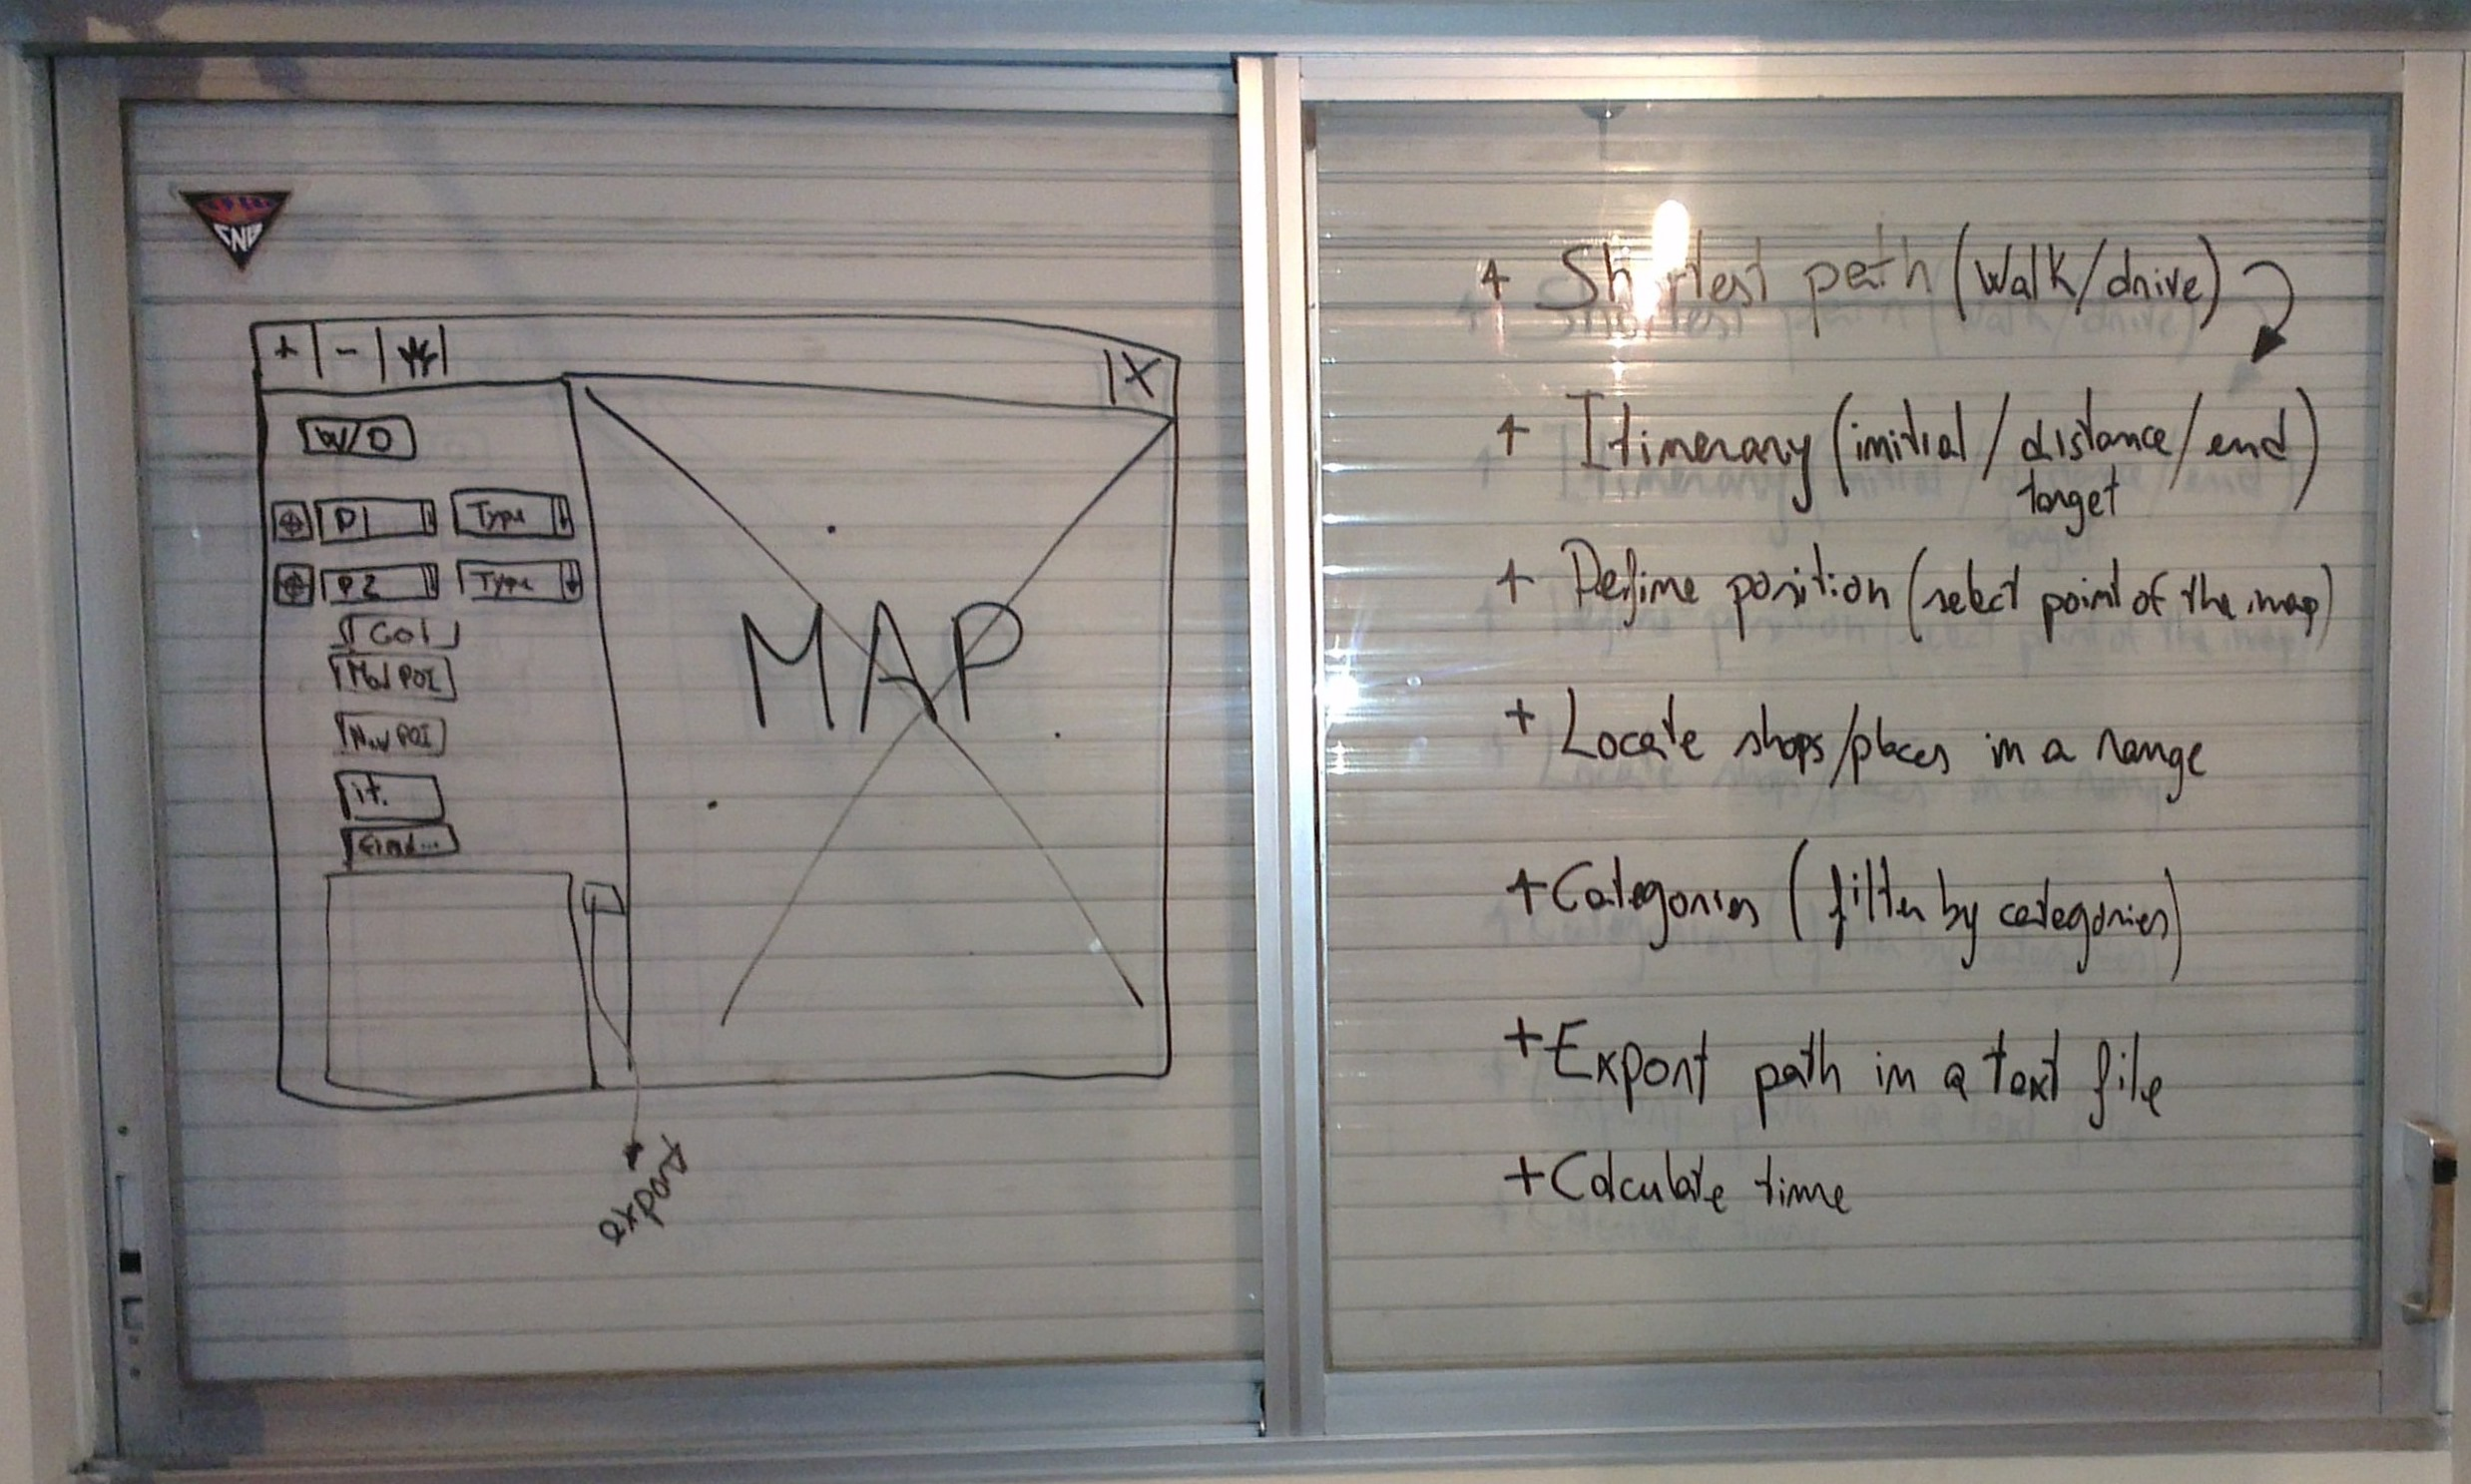
\includegraphics[width=0.7\textwidth]{windowBoard.jpg}
\caption{One of the team meeting. Window is used as a white board to gather all ideas/problems.}
\end{figure}

Concurrently we were looking for frameworks for managing software projects. We have found that \textit{Agile software development} methods as \textit{Scrum} could fit to iterative management development of our project, however as it requires a lot of knowledge, we left this framework to the future works and employed only general parts of this framework.

It is also important to establish the IDE and tools before starting to develop the project. On one hand, we assigned that \textit{open-source} Qt 5.0.1 OpenGL under Mingw compiler would be the appropriate platform because it is the last stable version of Qt and also because this open source developing environment allows us to create easier the graphical user interface and also render without adding by hard the OpenGL libraries. On the other hand, regarding to Matlab part, everything has been developed using the R2013a version of the software.

However, the previous software is not the only one used in the project. We supposed correctly the basic necessity to deal with data structures such as information related with roads, nodes, buildings or points of interest among other possible types (see section \textit{Methodology}). The options were to deal with this data coming from one, \textit{txt/xml} format files or similar or two, databases.
In both cases, Matlab and C++ implementation, the decision was to work with databases because of the amount of data and specially because is the easiest and fastest way to get detailed information of the structures without going over the whole structure in such cases as getting nodes shared by two different roads (see the \textit{Database} section).

Despite sharing the same EER schema, the database chosen for the Matlab part it is different from the one chosen for the C++ part. In this way, we decided to use PostgreSQL just because it is easier to make it work together with Matlab and using MySQL 5.6 with Qt which was more familiar to us. But also, the fact that we chose two different databases made us able to change between them if some problems of generation had been encountered. Note that we have used the correspondent browser of both platforms.

\subsection{Related works}

In order to be able to design a user-friendly and helpful application it is necessary to have a look to the current work, for instance GoogleMaps (https://maps.google.es/) or another non common but open-source solutions as MapGuide (http://mapguide.osgeo.org/) or OpenStreetMap (http://www.openstreetmap.org/). In fact checking the last solution we found the way to get most of the data required to render our map and to fulfil our databases. In addition, some of the information provided by this source was not used.

For user's information, OpenStreetMap data is stored topological data structure. Basically there are 4 data primitives as the basic components of \textit{OpenStreetMap}: nodes, ways, relations and tags. For us the first element was a main ingredient as geographical data source and the second element \textit{ways} represents relationship between various nodes. 

\textit{OpenStreetMap} has been a good provider of data but at the same time it has been necessary to adapt our database tables to the information obtained and in some cases to add some additional parameters because we have to take into account that this platform is not able to provide a route between two points, at least not in a direct way. For example, all elements as roads, forest, buildings, rivers, linear structures are represented as polygons of way elements, thus additional data filtering, subsets were used to prepare required datasets for implementation of project database.



\section{Application Design}
In this section is explained how the application was devised starting by the definition of the database as well as the analysis of the use cases taking into account the user and the design of the resultant graphical user interface prototype.

\subsection{Use cases}
In order to prototype the graphical user interface of both parts, we conceived the diagram of cases of use that the user could find. But, first of all, which use cases we have?

According to the statement provided we can identify the following cases:

\begin{itemize}
  \item Finding the shortest path between two nodes picked up from the screen providing information about distance and time depending on the way of transport.
  \item Finding the shortest path between three points including the same information.
  \item Locating a point of interest.
  \item Finding all points of interest of a specific type around one place.
  \item Creating/Modifying/Deleting a point of interest.
\end{itemize}

That also can be summarized in the following diagram:

\begin{figure}[h]
\centering
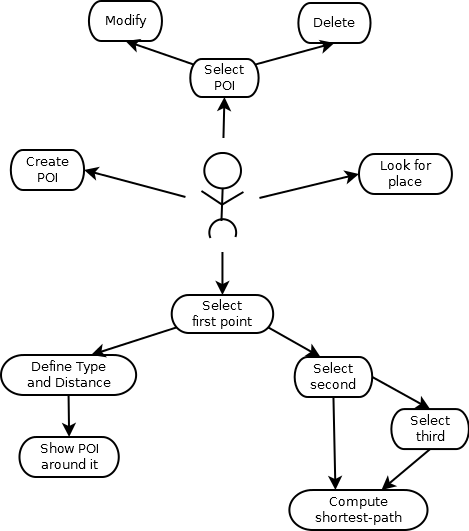
\includegraphics[width=0.6\textwidth]{use_cases.png}
\caption{Diagram of the use cases provided to the user}
\end{figure}

The user has to be able to select a point of interest which already exists, modify it and deleted from the database. But also has to be able to create a new point of interest and simply locate it on the map.

Once the user selects a point from the map, no matters if it is random position or a point of interest, we have the option to establish the distance we want to locate a specific type of points of interest around it. But also, we have the option to select a second or still a third point of interest for getting the shortest path.

\subsection{GUI prototype}
After defining the use cases that users have to be able to deal with, we can start prototyping the graphical user interface that is also common between the two implementations. To accomplish this hard task that can be adjusted to solve future requirements, we decided to divide the screen in 5 different relevant points explained below:

THE BROWSER: This section is marked with the number one in the following figure, first GUI prototype. Basically, it brings to the user the possibility to look for a point of interest that is already present in the database.

THE MAP: The zone shows a map able to be scaled (zoom in and zoom out) and reactive to mouse events in the whole surface.

SHORTEST-PATH: Number Three allows the user to establish a route between two or three points taking into account if he or she is moving by car or by foot. But also brings the possibility using the buttons located on the left, to look for a type of point of interest around one position.

POINTS OF INTEREST: Both Buttons located in number four allows the user to create a new point of interest or modify an existing one through a form.

ROUTE: Finally, number five the distance and time that the user will spend having selected some locations previously. Showing the turns and the distances between them. Also brings the possibility to download all this text in a \textit{txt} file.

\begin{figure}[h]
\centering
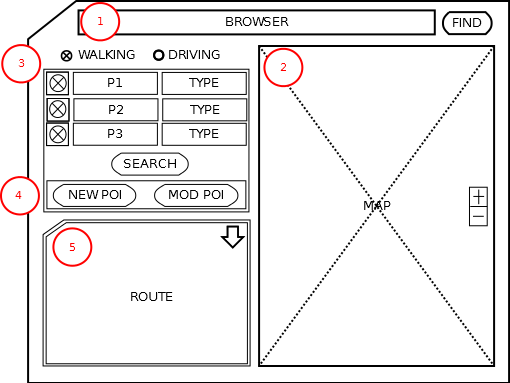
\includegraphics[width=0.7\textwidth]{Prototype.png}
\caption{First GUI prototype conceived at early stages of the design process}
\end{figure}

\subsection{Getting the data}
With the aim of creating a robust database where solving the problems proposed by the statement and in order to the maintain the wholeness of the data inside we have to consider the following statement:

\textit{"One map is composed by ROADS which in turn are composed by different NODES. However, a node could belong to more than one road which identifies an intersection between two roads. The only attributes necessary for a node would be a unique ID and the position of the node in a map defined by LATITUDE and LONGITUDE. In the same way all roads have the following attributes: A unique ID that identifies it, its NAME, a TYPE that describes if the road can be used by cars and finally, if it can be walked in both WAYS."}

Here, we can identify two tables, its attributes and the relation between them which can e defined as N:M because of the fact that one node can belong to multiple roads, and one road have multiple nodes. But also this relationship has to be defined taking into account the order the node has in the road that belongs to, giving an attribute of the relationship called ORDER.

On the other hand, the user has to be able to see the points of interest, create news, delete them and also modify the ones which already exist. We decided to create a table in the same schema without any relationship with the previous tables in order to maintain the isolation from the points updated all the time because it does not belong to any specific road.
The number of attributes considered from the very beginning for the points of interest (POI) table are: The ID and the position in LATITUDE and LONGITUDE, the NAME of the point, as well as the ADDRESS and the TYPE.

Taking into account the previous steps, we can see the result of the database in the following schema:

\begin{figure}[h]
\centering
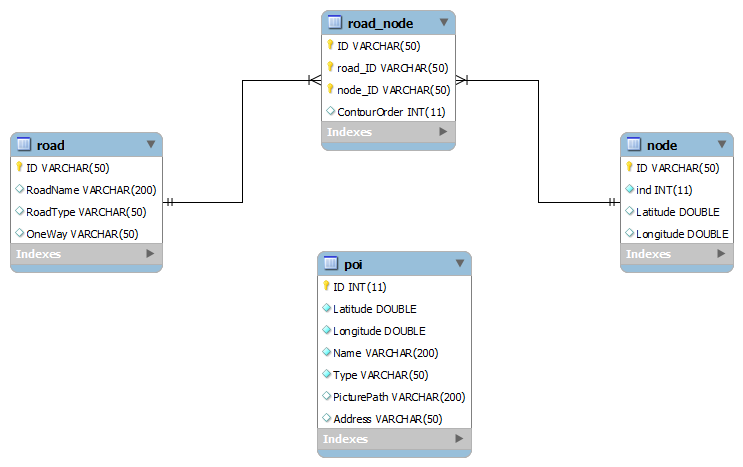
\includegraphics[width=0.6\textwidth]{EER_Diagram.png}
\caption{Diagram of the relational database model created during the design}
\label{fig:RelDBdiagram}
\end{figure}

Notice that part of the process of development and parsing of the data from OpenStreetMap into our databases was accomplished together with the rest of the groups.

\section{C++ Implementation}

The present section has been divided in two different parts: The first one explains how the map structure is created evolving the three basic classes, the correspondent adjacency matrix depending on the choice of the user (walking or driving), how the shortest path is calculated using Dijkstra's algorithm and the logic behind the management of the points of interest. During the second part, we will focus on how the data is shown and obtained directly from the screen and its process of normalization and denormalization, taking into account the different spatial coordinates we work with during the implementation. But also we will see how the graphical user interface provides the input/output to the user and how is managed.

\subsection{Creating the map}
The implementation of the application started with classes \textit{Node}, \textit{Road} and \textit{Map} according to the three tables already existing in the database and with the goal of loading all necessary points that composes the map of le Creusot in memory. However, at the same time, we wanted to take profit of the whole process storing all nodes that composes one road in the same structure. As a consequence, the map structure is a vector container that keeps as many pointers to road structures as number of roads are in the map. At the same time, each road is a vector container whose size is defined by the number of nodes that compose it. However, what is stored in the road structure are pointers to nodes.

\begin{lstlisting}
vector<Road*> myMap 	//Definition of map structure
vector<Node*> myRoad;	//Definition of road structure
\end{lstlisting}

Composing the following relationship:

\begin{figure}[h]
\centering
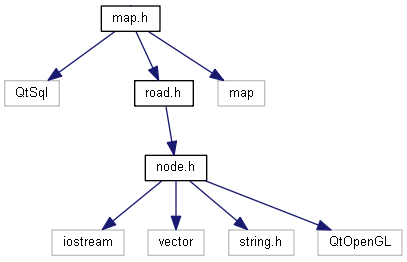
\includegraphics[width=0.6\textwidth]{map.png}
\caption{UML diagram of the three classes that composes the logic map: Map, Road and Node}
\end{figure}

As we can see our class map has dependencies with the class \textit{QtSQL}, necessary for making queries to the database but also contains a standard map structure. It is used in order to avoid checking node by node in some cases, a map that contains the node structures and its identifier is composed in the constructor. Finally, we can see some other dependences with standard libraries with \textit{QtOpenGL} the library that makes possible drawing the nodes that compose the map (explained in detail in the next section).

\subsection{The shortest path}


\subsubsection{Dijkstra's algorithm}

\subsubsection{The adjacency matrix}
The following section describes a specific method of the \textit{map} class that allows us to create an adjacency matrix of dimensions NxN where N is the total amount of nodes that composes the map. This matrix will be used to calculate the shortest path between two or more points in the map. Such matrix is generated according to the method of transport chosen by the user. For instance, we can not drive in both senses in all roads or driving in a foot way.

First of all, the structure is allocated in memory and initialized to the maximum distance in all positions, in our case 999 units, and 0 in the diagonal of the squared matrix. Then, the rest of the matrix is filed taking into account the distance between the nodes identified by the index of the rows and columns of the matrix. From this point, the only thing we have to do is to go over the map structure checking which nodes are consecutive meaning that exists a connection between them. In this way, the position $M_{adj}(1,2)$ would contain the distance between node 1 and node 2. But what happens with the position $M_{adj}(2,1)$? This position contains the same distance if and only if the road is two ways, fact that can be checked querying the attribute \textit{oneWay} located in table \textit{Roads} in the database. 
We can also take into account querying the database, if a road is a foot way or not and calculate the appropriate distance.
On the other hand, people can work in both senses and also use all king of roads, so we can generate the adjacency matrix in the same way without the restrictions explained above.

Notice that in order to calculate the distance between two nodes the method \textit{distNode()} was implemented in class \textit{node } following the formula of the euclidean distance. 

\clearpage
\section{Matlab Implementation}
       
In this section the project implementation using Matlab is discussed and presented. Most of the concepts are reused from C++ source code as the preservation of consistency between two different sources was one of the purposes. Thus here, only the differences are presented and discussed.

\subsection{Getting the data}

As it was mentioned before, in Matlab implementation we have chosen to use \textit{PostgreSQL} database, since the whole process (installing additional drivers for Matlab, making connectors, etc.) was more user friendly and time efficient. However, the database schema/structure and all data were the same between MySQL and PostgreSQL implementations (see figure: ~\ref{fig:RelDBdiagram}).

The first difference comes in fact that variables in Matlab can be not even created, but as well saved and loaded in Matlab's data structure \textit{.mat} files. This allowed us to come to the solution where the connection to external data source (database) is made only one time for creating appropriate data structures/class objects (discussed in next section). As in Matlab project part queries to database are used only one, the program end-user does not need to have database and driver installed, because afterwards all calculations are created using generated data structures from .mat files.

\subsection{Data Structure}

The second important question which had to be answered - the types of data structures in Matlab.
Since by itself Matlab has a lot of different data types from which the \textit{struct} objects can be created, we have decided to create own object classes with required properties and methods. The reader should note, that there a lot of differences between Matlab and other OOP languages, thus all of those will not be discussed since all information can be found in the web.\footnote{
\url{http://www.mathworks.fr/fr/help/matlab/matlab_oop/matlab-vs-other-oo-languages.html}
}

Another faced issue was the fact that the Matlab is not so flexible as C++ with passing objects by pointer or reference. Since we would like to avoid creating a copies of original objects in functions, we found that \textit{handle} classes in Matlab can be created, where class constructor returns a handle object that is a reference to the object created. In this way, using such objects in functions, MATLAB copies just the handle and access its data indirectly.

As in C++ implementation, classes for representing the \textit{node}, \textit{road} and \textit{map} were created.

\begin{figure}[!h]
\centering
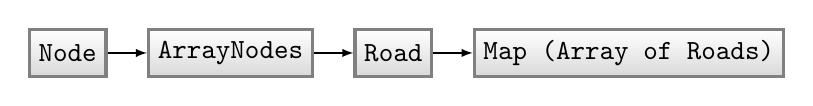
\begin{tikzpicture}[node distance=5mm,
terminal/.style={
% The shape:
rectangle,
minimum size=6mm,
% The rest
very thick,draw=black!50,
top color=white,bottom color=black!15,
font=\ttfamily}]

\node (Node) [terminal] {Node};
\node (ArrNode) [terminal,right=of Node] {ArrayNodes};
\node (Road) [terminal,right=of ArrNode] {Road};
\node (Map) [terminal,right=of Road] {Map (Array of Roads)};
\path
(Node) edge[-latex] (ArrNode) % simple edges
(ArrNode) edge[-latex] (Road)
(Road) edge[-latex] (Map);

\end{tikzpicture}
\caption{Simplified diagram of relationship of a classes}
\end{figure}

As opposite to C++ implementation, here the additional class \textit{ArrayNodes} was created. This was done with intention to vectorize some methods, since Matlab is optimized for operations involving matrices and vectors. Of course, it was possible to implement such methods directly to the road class, though the recent method was chosen to emphasize that methods are only related with the Array of \textit{Nodes}.

Notwithstanding our option, the user could find an alternative or better data structure for the same goal.
For example, together with the team we discussed another options such as keeping data in project in the same way as in kept in the database: roads and nodes and the dictionary (linking table) between roads and nodes. Such structure would have it's advantage that various connections between roads and nodes would be easier accessible, e.g. it would be possible to get all roads where node \textit{X} is included and vice versa, while the our methodology requires additional methods to get the same results. 

% % matlab
% % Shortest Path
\subsection{The shortest path}
% % % % % % % % % % % % % % % % % % % % % % % % % % % % % % %
% projection figure
\begin{figure}[!h]
\centering
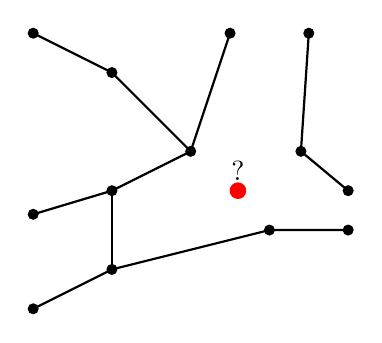
\begin{tikzpicture}[
	%	style def
    scale=1,
    important line/.style={thick},
    every node/.style={color=black}
    ]
	
	% demo connection of nodes
	\draw[important line] (0,1) coordinate (a1) -- (1,1.5) coordinate (a2) -- (3,2) coordinate (a3) -- (4,2) coordinate (a4);
	\draw[important line] (0,2.2)coordinate (C2) -- (1,2.5) coordinate (D) -- (2,3) coordinate (E) -- (2.5, 4.5) coordinate (F);
	\draw[important line] (a2)--(D) ;
	\draw[important line] (E)--(1,4) coordinate (G) -- (0,4.5) coordinate (H);
    \draw[important line] (3.5,4.5)coordinate (I) -- (3.4,3) coordinate (J)  --  (4,2.5) coordinate (K) ;
    \fill[black] 
        		 (a1) circle (2pt)
    			 (a2) circle (2pt)
    			 (a3) circle (2pt)
    			 (a4) circle (2pt)
    			 (C2) circle (2pt)
    			 (D) circle (2pt)
    			 (E) circle (2pt)
    			 (F) circle (2pt)
    			 (G) circle (2pt)
    			 (H) circle (2pt)
    			 (I) circle (2pt)
    			 (J) circle (2pt)
    			 (K) circle (2pt);
    %circle representing user input			 
    \fill[red] (2.6,2.5) circle (3pt) node[above] {$?$};
\end{tikzpicture}
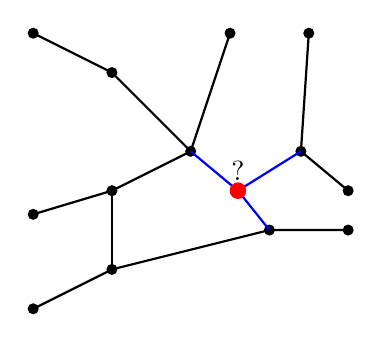
\begin{tikzpicture}[
	%	style def
    scale=1,
    important line/.style={thick},
    every node/.style={color=black}
    ]
	
	% demo connection of nodes
	\draw[important line] (0,1) coordinate (a1) -- (1,1.5) coordinate (a2) -- (3,2) coordinate (a3) -- (4,2) coordinate (a4);
	\draw[important line] (0,2.2)coordinate (C2) -- (1,2.5) coordinate (D) -- (2,3) coordinate (E) -- (2.5, 4.5) coordinate (F);
	\draw[important line] (a2)--(D) ;
	\draw[important line] (E)--(1,4) coordinate (G) -- (0,4.5) coordinate (H);
    \draw[important line] (3.5,4.5)coordinate (I) -- (3.4,3) coordinate (J)  --  (4,2.5) coordinate (K) ;
    \fill[black] 
        		 (a1) circle (2pt)
    			 (a2) circle (2pt)
    			 (a3) circle (2pt)
    			 (a4) circle (2pt)
    			 (C2) circle (2pt)
    			 (D) circle (2pt)
    			 (E) circle (2pt)
    			 (F) circle (2pt)
    			 (G) circle (2pt)
    			 (H) circle (2pt)
    			 (I) circle (2pt)
    			 (J) circle (2pt)
    			 (K) circle (2pt);
    %circle representing user input			 
    \fill[red] (2.6,2.5) coordinate(user) circle (2pt) ;
    			     

    \draw[important line, blue] (user) -- (a3);
    \draw[important line, blue] (user) -- (E);
    \draw[important line, blue] (user) -- (J);
    %connecting closest nodes
        %circle representing user input			 
        \fill[red] (user) circle (3pt) node[above] {$?$};
    
    
\end{tikzpicture}
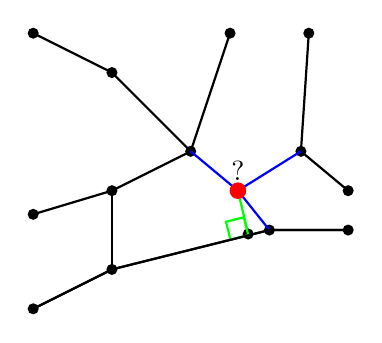
\begin{tikzpicture}[
	%	style def
    scale=1,
    important line/.style={thick},
    every node/.style={color=black}
    ]
	
	% demo connection of nodes
	\draw[important line] (0,1) coordinate (a1) -- (1,1.5) coordinate (a2) -- (3,2) coordinate (a3) -- (4,2) coordinate (a4);
	\draw[important line] (0,2.2)coordinate (C2) -- (1,2.5) coordinate (D) -- (2,3) coordinate (E) -- (2.5, 4.5) coordinate (F);
	\draw[important line] (a2)--(D) ;
	\draw[important line] (E)--(1,4) coordinate (G) -- (0,4.5) coordinate (H);
    \draw[important line] (3.5,4.5)coordinate (I) -- (3.4,3) coordinate (J)  --  (4,2.5) coordinate (K) ;
    \fill[black] 
        		 (a1) circle (2pt)
    			 (a2) circle (2pt)
    			 (a3) circle (2pt)
    			 (a4) circle (2pt)
    			 (C2) circle (2pt)
    			 (D) circle (2pt)
    			 (E) circle (2pt)
    			 (F) circle (2pt)
    			 (G) circle (2pt)
    			 (H) circle (2pt)
    			 (I) circle (2pt)
    			 (J) circle (2pt)
    			 (K) circle (2pt);
   %circle representing user input			 
    \fill[red] (2.6,2.5) coordinate(user) circle (2pt) ;
    			     
	%connecting closest nodes
    \draw[important line, blue] (user) -- (a3);
    \draw[important line, blue] (user) -- (E);
    \draw[important line, blue] (user) -- (J);
    % projection
    \draw[important line, green] (user) -- (2.73, 1.95) coordinate (intersect);
    \fill[black] (intersect) circle (2pt) ;
    
    \draw[important line, green, ] (intersect)+(-0.14,0.07) node[minimum size=0.1cm,draw,green, rotate =14]{};
    %circle representing user input			 
    \fill[red] (user) circle (3pt) node[above] {$?$};
    \draw[important line] (a1) -- (a2) -- (a3) -- (a4);    
\end{tikzpicture}

\caption{Random point projections}
\end{figure}
\end{document}



